\chapter{บทนำสู่การเรียนรู้เชิงสถิติและปัญญาประดิษฐ์} 
\label{CH1_Intro}
\section{คำอธิบายรายวิชา}
ภาพรวมของการเรียนรู้เชิงสถิติ พื้นฐานสถิติสำหรับการเรียนรู้ การเรียนรู้แบบมีผู้สอน การเรียนรู้แบบไม่มีผู้สอน เทคนิคการเรียนรู้ของเครื่องเชิงสถิติ เช่น การถดถอยเชิงเส้น การถดถอยโลจิสติค ต้นไม้ตัดสินใจ การสุ่มป่าไม้ และนาอีฟเบส์ เป็นต้น การประเมินประสิทธิภาพของโมเดล


%##########################################
\section{ความสำคัญของสถิติศาสตร์ในปัญญาประดิษฐ์}
สถิติศาสตร์เปรียบเสมือนหัวใจสำคัญของปัญญาประดิษฐ์ (Artificial Intelligence: AI) โดยทำหน้าที่เป็นรากฐานทฤษฎีที่ช่วยให้ระบบคอมพิวเตอร์สามารถเรียนรู้จากข้อมูล (Data-Driven Learning) ได้อย่างมีประสิทธิภาพ ในยุคปัจจุบันที่ข้อมูลมีความซับซ้อนและมีขนาดใหญ่ (Big Data) หลักการทางสถิติช่วยให้ AI สามารถแยกแยะ ``รูปแบบที่แท้จริง'' (Pattern) ออกจาก ``ความผันแปร'' (Noise) ของข้อมูลได้ ซึ่งเป็นสิ่งจำเป็นอย่างยิ่งสำหรับการสร้างโมเดลที่แม่นยำ ไม่ว่าจะเป็นการใช้ทฤษฎีความน่าจะเป็น (Probability Theory) เพื่อการตัดสินใจภายใต้สถานการณ์ที่ไม่แน่นอน หรือการใช้วิธีการอนุมานเชิงสถิติ (Statistical Inference) เพื่อพยากรณ์แนวโน้มในอนาคต หากปราศจากสถิติศาสตร์ AI จะเป็นเพียงอัลกอริทึมที่ขาดความสามารถในการทำความเข้าใจบริบทและความน่าเชื่อถือของข้อมูล

\begin{figure}[h]
	\centering
	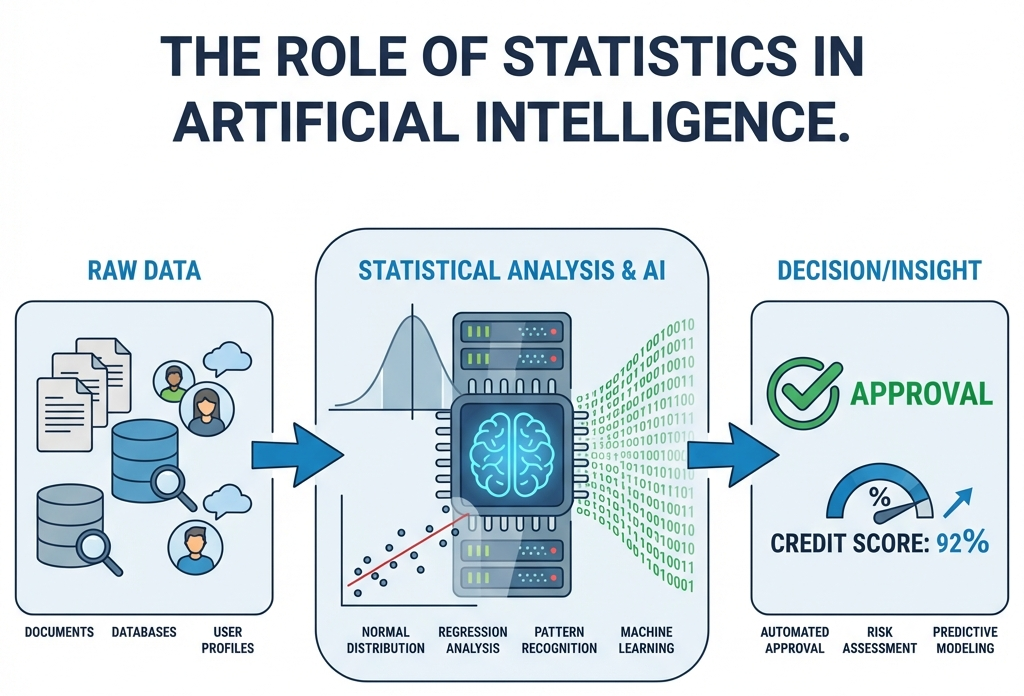
\includegraphics[width=0.8\textwidth]{example_ai_stat.png}
	\caption{แผนภาพแสดงบทบาทของสถิติศาสตร์ในการเปลี่ยนข้อมูลดิบ (Raw Data) ให้เป็นความรู้ (Insight) เพื่อการตัดสินใจในระบบ AI}
	\label{fig:stat_in_ai}
\end{figure}

ตัวอย่างกรณีศึกษาที่ชัดเจนคือการประยุกต์ใช้ใน \textbf{อุตสาหกรรมการเงินและการธนาคาร} เช่น ระบบการให้คะแนนเครดิต (Credit Scoring) ซึ่งธนาคารใช้ AI ในการประเมินความเสี่ยงของผู้กู้ ระบบเหล่านี้ใช้เทคนิคทางสถิติ เช่น การถดถอยโลจิสติค (Logistic Regression) หรือการจำแนกกลุ่ม (Classification) เพื่อวิเคราะห์ประวัติทางการเงินและพฤติกรรมการใช้จ่าย จากนั้นจึงคำนวณออกมาเป็น ``ความน่าจะเป็น'' ที่ลูกค้าจะผิดนัดชำระหนี้ การใช้สถิติเข้ามาจับช่วยลดความลำเอียง (Bias) ของมนุษย์และเพิ่มความแม่นยำในการอนุมัติสินเชื่อได้อย่างมหาศาล ดังแสดงในภาพประกอบ \ref{fig:stat_in_ai} ที่แสดงกระบวนการแปลงข้อมูลดิบให้เป็นข้อมูลเชิงลึกผ่านโมเดลทางสถิติ




%##########################################
\section{บทบาทหลักของสถิติศาสตร์ในปัญญาประดิษฐ์}
ในการพัฒนาโมเดลการเรียนรู้ของเครื่อง (Machine Learning: ML) ในปัญญาประดิษฐ์ที่มีประสิทธิภาพ สถิติศาสตร์ไม่ได้ทำหน้าที่เพียงแค่การสรุปผลจากข้อมูลเพียงเท่านั้น แต่ยังเป็นกลไกหลักในการขับเคลื่อนกระบวนการเรียนรู้ของเครื่องในทุกขั้นตอน หากพิจารณาตามกระบวนการทำงานด้านวิทยาการข้อมูล (Data Science) เราสามารถจำแนกบทบาทของสถิติศาสตร์ออกเป็นหัวข้อหลักที่สำคัญได้แก่ \textbf{การทำความเข้าใจและอธิบายข้อมูล (Data Understanding)} ซึ่งเป็นการเตรียมความพร้อมของข้อมูล \textbf{การสร้างโมเดล (Model Formulation)} ซึ่งเป็นขั้นตอนการเรียนรู้รูปแบบของข้อมูล และ \textbf{การประเมินประสิทธิภาพโมเดล (Model Evaluation)} ซึ่งเป็นการตรวจสอบความถูกต้องของโมเดล โดยแต่ละบทบาทแสดงรายละเอียดดังนี้



\subsection{การทำความเข้าใจและอธิบายข้อมูล} 
การทำความเข้าใจและอธิบายข้อมูล (Data Understanding and Description) หรือที่รู้จักกันในชื่อ Exploratory Data Analysis (EDA) เป็นกระบวนการแรกที่สำคัญที่สุดในการวิเคราะห์ข้อมูลเพื่อเตรียมความพร้อมสำหรับอัลกอริทึม AI เป้าหมายไม่ใช่เพียงการคำนวณค่าสถิติพื้นฐาน แต่คือการ "ฟังเสียงของข้อมูล" เพื่อค้นหารูปแบบที่ซ่อนอยู่ (Hidden Patterns) ความสัมพันธ์ระหว่างตัวแปร (Correlations) และที่สำคัญที่สุดคือการตรวจจับความผิดปกติ (Anomalies) ที่อาจส่งผลกระทบต่อความแม่นยำของโมเดล การใช้สถิติศาสตร์ในขั้นตอนนี้จะช่วยให้นักวิทยาศาสตร์ข้อมูลสามารถตัดสินใจเลือกเทคนิคการประมวลผล (Preprocessing) ที่เหมาะสมที่สุดสำหรับข้อมูลแต่ละชุด เพื่อให้เห็นภาพชัดเจน สามารถพิจารณากรณีศึกษาดังต่อไปนี้

\begin{itemize}
	\item \textbf{กรณีศึกษาที่ 1: การตรวจจับความผิดปกติในข้อมูลทางการแพทย์ (Medical Anomaly Detection)}
	
	ในระบบเฝ้าระวังผู้ป่วยอัตโนมัติโดยใช้โมเดลการเรียนรู้ของเครื่องสำหรับจำแนกระหว่างสัญญาณชีพปกติและสัญญาณภาวะวิกฤต การใช้ค่าสถิติพื้นฐานเช่น \textbf{ค่าเฉลี่ย (Mean)} และ \textbf{ส่วนเบี่ยงเบนมาตรฐาน (Standard Deviation: SD)} ช่วยให้เรากำหนด "ขอบเขตปกติ" (Normal Threshold) ของอัตราการเต้นของหัวใจได้ ข้อมูลที่อยู่นอกเหนือขอบเขตนี้ (Outliers) จะถูกระบุว่าเป็นความผิดปกติที่ต้องแจ้งเตือนแพทย์ทันที ดังแสดงในภาพประกอบ \ref{fig:outlier_detect} ซึ่งจุดสีแดงแสดงถึงค่าที่ผิดปกติอย่างชัดเจนเมื่อเทียบกับการกระจายตัวของข้อมูลส่วนใหญ่
	
	\begin{figure}[h]
		\centering
		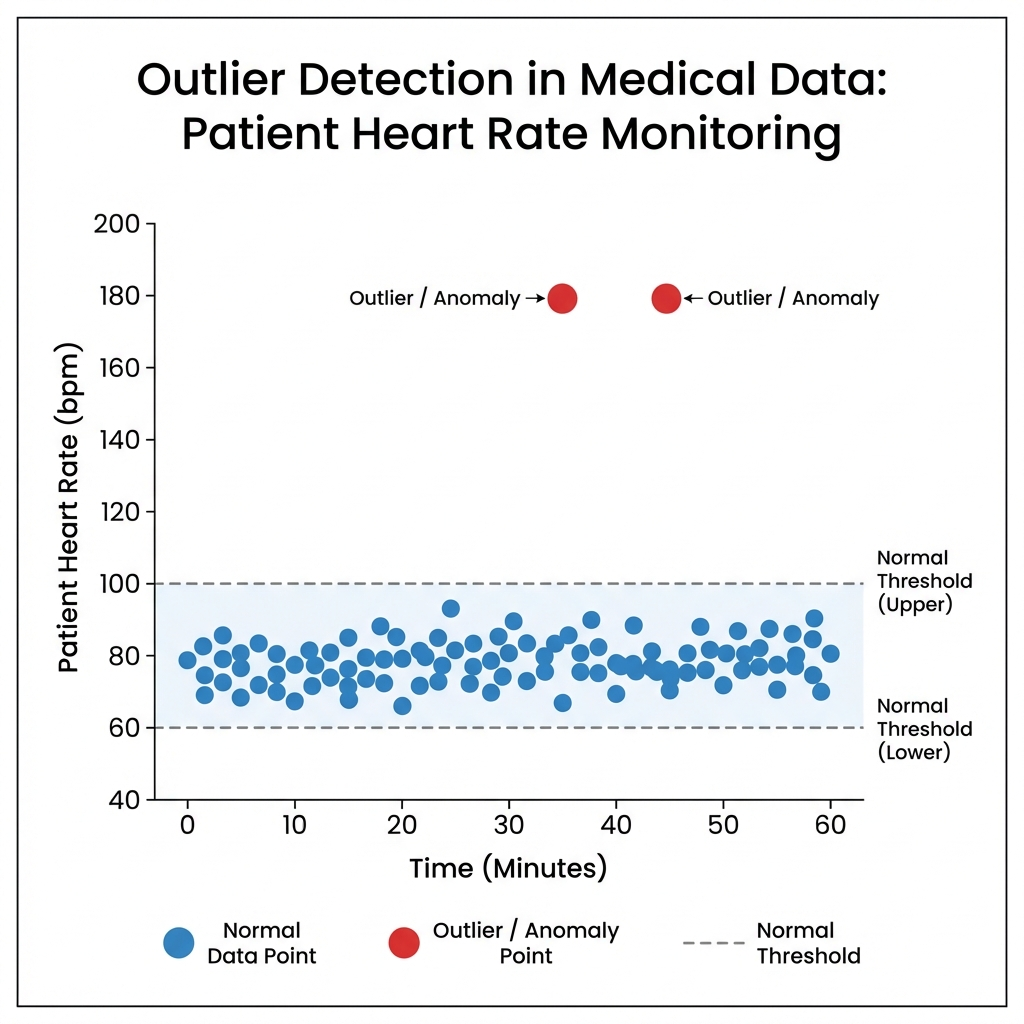
\includegraphics[width=0.7\textwidth]{outlier_detection_example.png} 
		\caption{การใช้หลักการทางสถิติเพื่อตรวจจับค่าผิดปกติ (Outliers) ในสัญญาณชีพผู้ป่วย}
		\label{fig:outlier_detect}
	\end{figure}
	
	\item \textbf{กรณีศึกษาที่ 2: การวิเคราะห์พฤติกรรมการซื้อสินค้าของผู้บริโภค (Customer Behavior Analysis)}
	
	เมื่อต้องการสร้างระบบแนะนำสินค้า (Recommender System) ข้อมูลรายได้หรือยอดซื้อของลูกค้ามักจะไม่มีการแจกแจงแบบปกติ (Normal Distribution) แต่มักจะมีการแจกแจงแบบ \textbf{เบ้ขวา (Right-Skewed Distribution)} กล่าวคือ ลูกค้าส่วนใหญ่มียอดซื้อปานกลาง (ส่วนยอดกราฟ) แต่มีลูกค้ากลุ่มน้อยที่มียอดซื้อสูงมาก (หางกราฟยาวไปทางขวา) ในกรณีเช่นนี้ การใช้ "ค่าเฉลี่ย" (Mean) จะถูกดึงให้สูงขึ้นตามลูกค้ากระเป๋าหนัก ทำให้ไม่ได้ตัวแทนข้อมูลที่แท้จริง ดังนั้นสถิติศาสตร์จึงแนะนำให้ใช้ \textbf{ค่ามัธยฐาน (Median)} หรือ \textbf{ฐานนิยม (Mode)} เป็นตัวแทนข้อมูลที่ดีกว่าในการทำความเข้าใจพฤติกรรมลูกค้าส่วนใหญ่ ดังภาพประกอบ \ref{fig:skewed_dist}
	
	\begin{figure}[h]
		\centering
		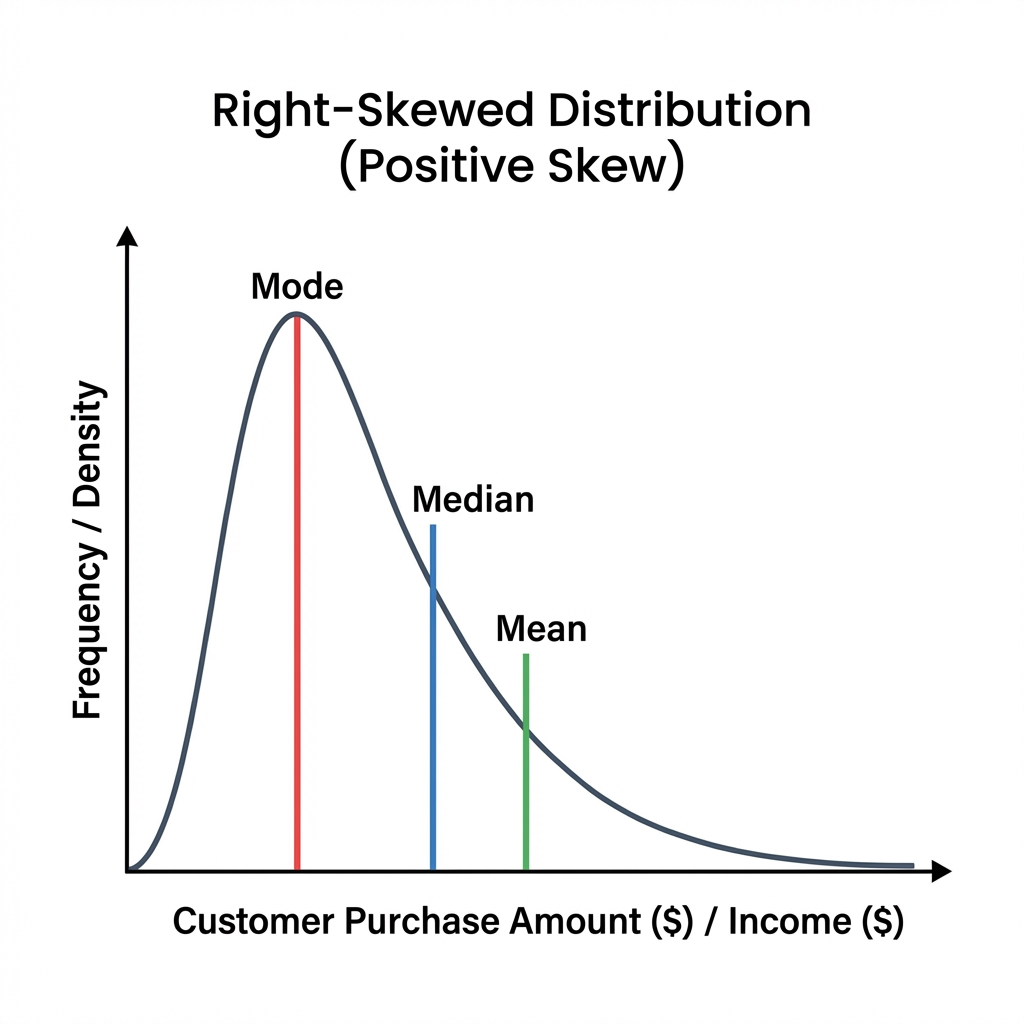
\includegraphics[width=0.5\textwidth]{skewed_distribution_example.png} 
		\caption{ลักษณะการแจกแจงข้อมูลแบบเบ้ขวา (Positive Skew) ที่พบได้บ่อยในข้อมูลพฤติกรรมผู้บริโภค}
		\label{fig:skewed_dist}
	\end{figure}
\end{itemize}

\begin{exmp}
	บริษัทอสังหาริมทรัพย์ต้องการสร้างระบบอัจฉริยะโดยใช้โมเดลการเรียนรู้ของเครื่องเพื่อประเมินราคาบ้านในกรุงเทพมหานครมีข้อมูลบ้าน 10 หลัง ประกอบด้วยตัวแปร แสดงดังตาราง \ref{Ex_home} 
	
	\begin{table}[h!]
		\centering
		\caption{ข้อมูลตัวอย่างราคาบ้านและปัจจัยที่เกี่ยวข้องจำนวน 10 หลัง}
		\label{Ex_home}
		\begin{tabular}{|c|c|c|c|c|c|}
			\hline
			\textbf{ลำดับ} & \textbf{พื้นที่ใช้สอย (ตร.ม.)} & \textbf{จำนวนห้องนอน} & \textbf{ระยะห่าง BTS (กม.)} & \textbf{อายุบ้าน (ปี)} & \textbf{ราคา (ล้านบาท)} \\ \hline
			1 & 50 & 1 & 0.5 & 5 & 3.5 \\ \hline
			2 & 80 & 2 & 1.2 & 8 & 5.2 \\ \hline
			3 & 120 & 3 & 2.5 & 10 & 6.8 \\ \hline
			4 & 45 & 1 & 0.2 & 2 & 4.0 \\ \hline
			5 & 60 & 2 & 5.0 & 15 & 2.8 \\ \hline
			6 & 200 & 4 & 3.0 & 5 & 12.5 \\ \hline
			7 & 35 & 1 & 0.1 & 1 & 3.8 \\ \hline
			8 & 90 & 3 & 1.5 & 20 & 4.5 \\ \hline
			9 & 150 & 3 & 4.0 & 12 & 7.5 \\ \hline
			10 & 75 & 2 & 0.8 & 6 & 4.9 \\ \hline
		\end{tabular}
	\end{table}
	
	
	การวิเคราะห์โดยใช้สถิติเชิงพรรณนา ประกอบด้วยดังนี้
	
	การวิเคราะห์ข้อมูลตารางข้างต้น โดยใช้ภาษา Python แสดงดังภาพ \ref{Ex_home_python_combined}
	
	\begin{figure}[h] \label{Ex_home_python_combined}
		\centering
		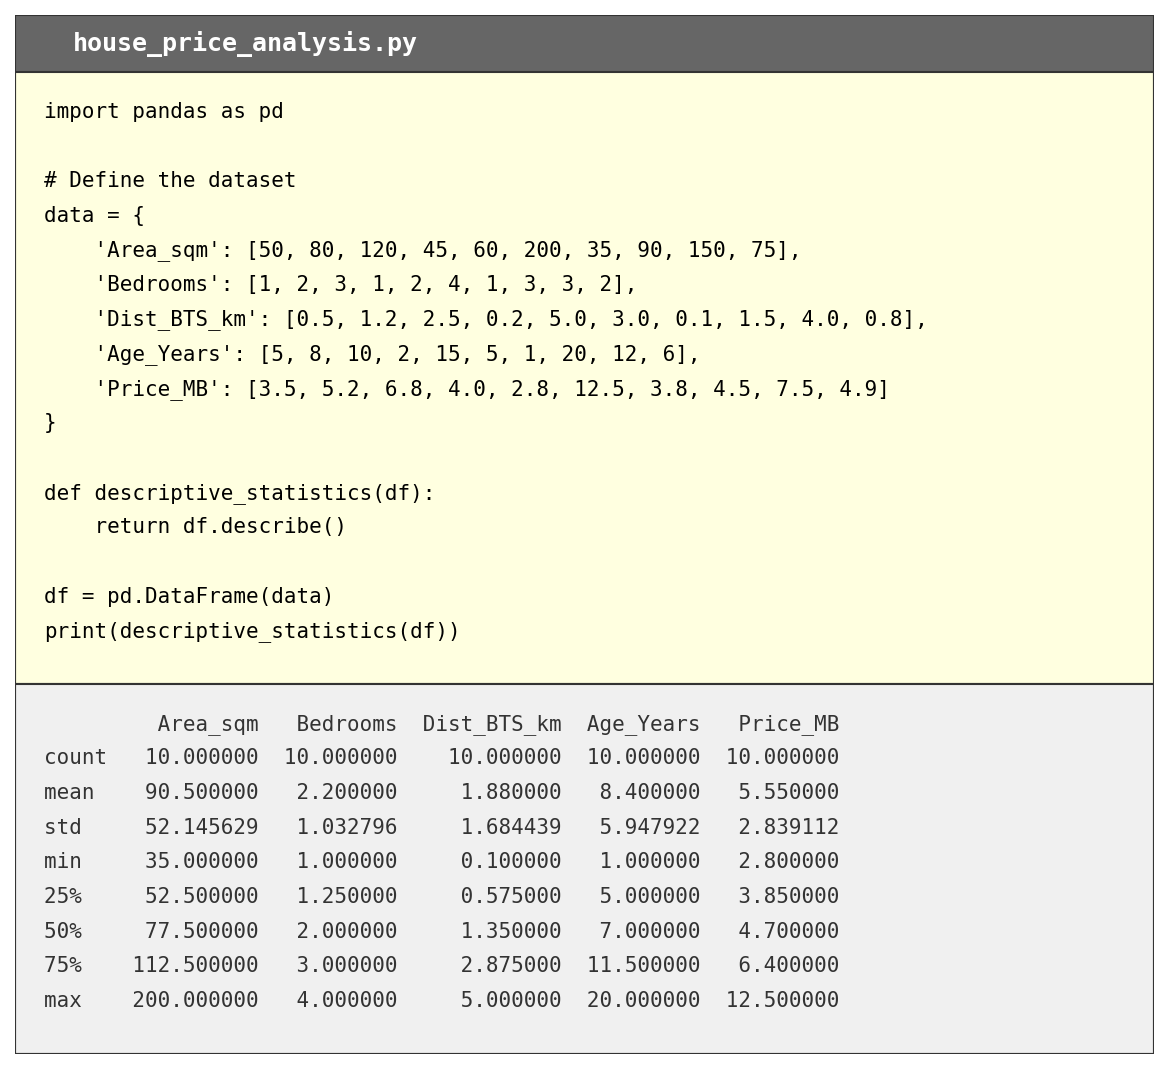
\includegraphics[scale=0.7]{CH1_python_combined.png}
		\caption{Python code และผลลัพธ์การคำนวณสถิติเชิงพรรณนา}
	\end{figure}
	
	\begin{figure}[h] \label{Ex_home_scatter_combined}
		\centering
		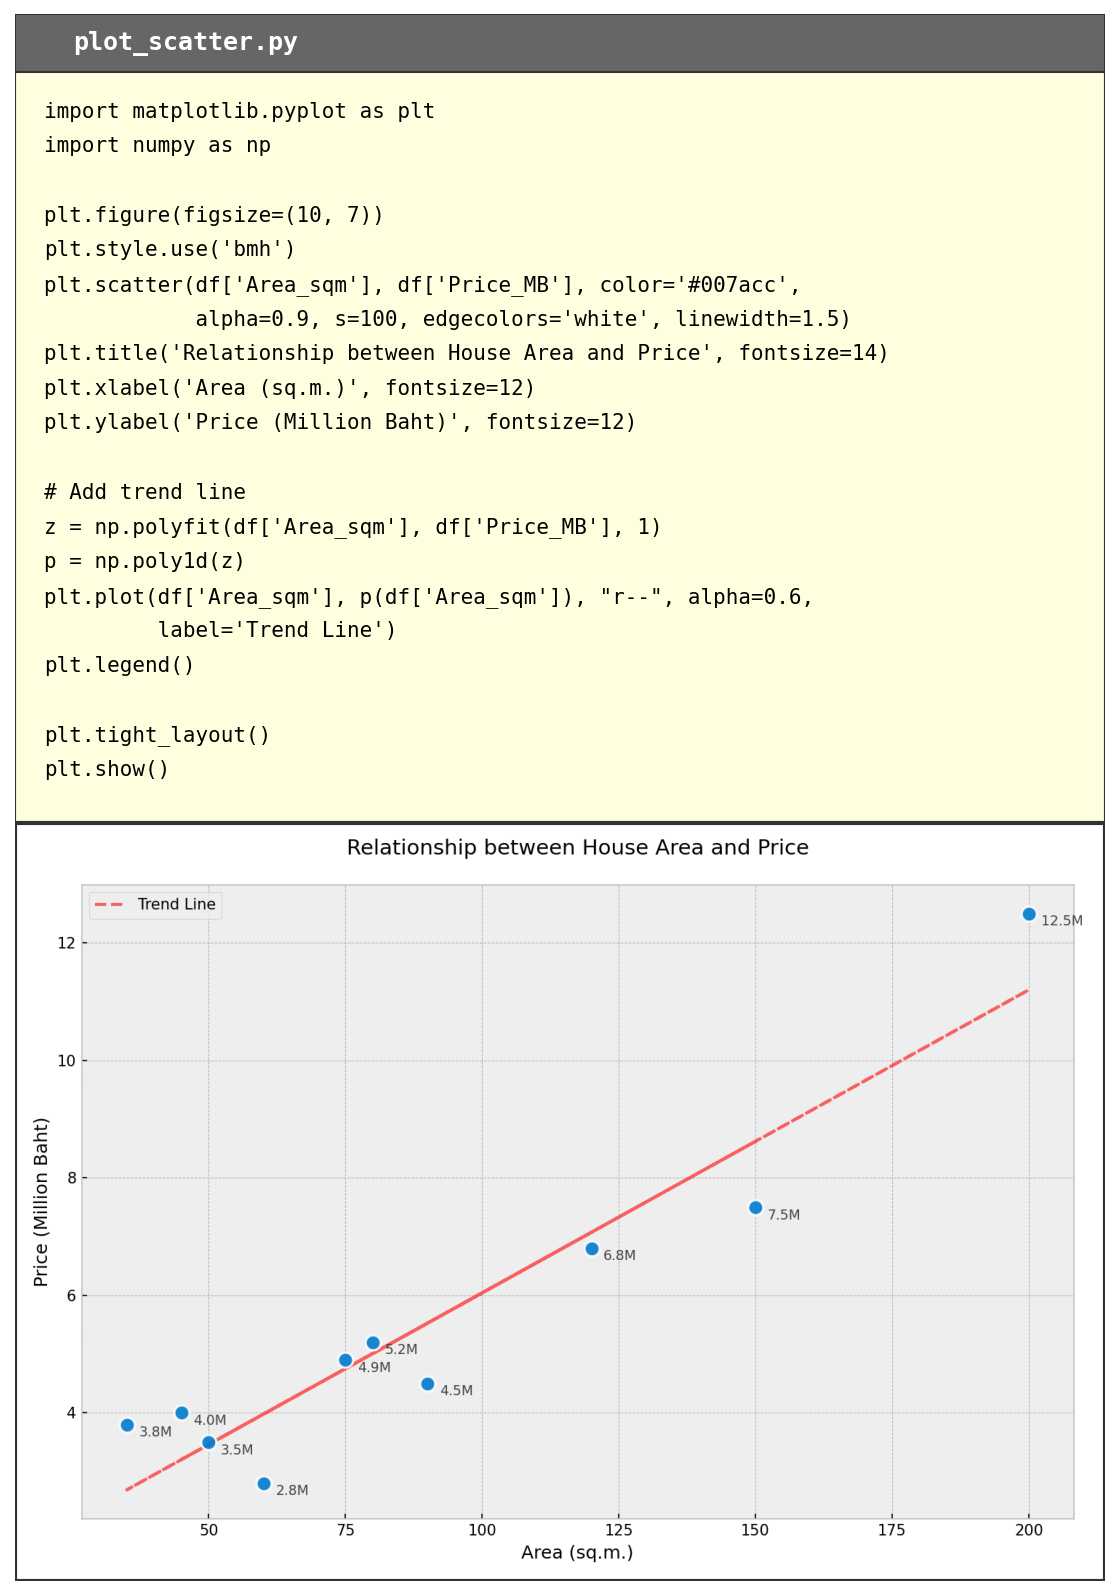
\includegraphics[scale=0.7]{CH1_scatter_combined.png}
		\caption{Python code สำหรับการสร้างกราฟและผลลัพธ์แผนภาพการกระจาย (Scatter Plot)}
	\end{figure}
	
	
\end{exmp}

\subsection{การสร้างโมเดล}

การสร้างโมเดล (Model Formulation หรือ Model Building) เป็นขั้นตอนหลักที่สองในกระบวนการวิเคราะห์ข้อมูลด้วย Machine Learning ซึ่งตามมาหลังจากการทำความเข้าใจและอธิบายข้อมูล ในขั้นตอนนี้ เราจะนำความรู้และข้อมูลเชิงลึก (Insights) ที่ได้จากการวิเคราะห์เบื้องต้น (Exploratory Data Analysis) มาใช้ในการสร้าง ``ตัวแบบทางคณิตศาสตร์'' (Mathematical Model) ที่สามารถเรียนรู้รูปแบบจากข้อมูลและทำนายผลลัพธ์ได้อย่างแม่นยำ

\textbf{หัวใจสำคัญของการสร้างโมเดล} คือการหาฟังก์ชัน $f(\mathbf{x}; \boldsymbol{\theta})$ ที่สามารถอธิบายความสัมพันธ์ระหว่าง \textbf{ตัวแปรอิสระ} (Input Features) $\mathbf{x} = (x_1, x_2, \ldots, x_k)$ เช่น อายุ น้ำหนัก ความดันโลหิต กับ \textbf{ตัวแปรตาม} (Target Variable) $Y$ เช่น ผลการวินิจฉัยโรค ระยะเวลารักษาหาย โดยผ่านกระบวนการ ``การเรียนรู้พารามิเตอร์'' (Parameter Learning) เพื่อหาค่า $\boldsymbol{\theta}$ ที่เหมาะสมที่สุด (Optimal Parameters)

\begin{myBox}[]{องค์ประกอบหลักของการสร้างโมเดล}{}
การสร้างโมเดลเชิงสถิติสำหรับ AI ประกอบด้วย 4 ขั้นตอนหลัก ดังนี้

\begin{enumerate}
	\item \textbf{การเลือกรูปแบบโมเดล (Model Selection)} - การเลือกโครงสร้างทางคณิตศาสตร์ที่เหมาะสมกับลักษณะของข้อมูลและวัตถุประสงค์ของปัญหา โดยพิจารณาจากประเภทของตัวแปรตาม (ต่อเนื่องหรือไม่ต่อเนื่อง) ความสัมพันธ์ระหว่างตัวแปร (เชิงเส้นหรือไม่เชิงเส้น) และขนาดคุณภาพของข้อมูล
	
	\item \textbf{การเรียนรู้พารามิเตอร์ (Parameter Learning)} - กระบวนการหาค่าพารามิเตอร์ที่เหมาะสมที่สุดโดยใช้เทคนิคทางสถิติ เช่น วิธีกำลังสองน้อยที่สุด (Ordinary Least Squares - OLS) สำหรับการถดถอยเชิงเส้น วิธีภาวะน่าจะเป็นสูงสุด (Maximum Likelihood Estimation - MLE) สำหรับการถดถอยโลจิสติค หรือ วิธี Gradient Descent สำหรับโมเดลที่ซับซ้อน
	
	\item \textbf{การประเมินและตรวจสอบโมเดล (Model Validation)} - การตรวจสอบประสิทธิภาพของโมเดลด้วยข้อมูลที่ยังไม่เคยเห็น (Test Data) โดยใช้ตัวชี้วัดที่เหมาะสม เช่น Mean Squared Error (MSE), $R^2$ สำหรับการถดถอย หรือ Accuracy, Precision, Recall สำหรับการจำแนกประเภท
	
	\item \textbf{การปรับแต่งและเพิ่มประสิทธิภาพ (Model Tuning)} - การปรับปรุงโมเดลเพื่อหลีกเลี่ยงปัญหา Overfitting (โมเดลจำข้อมูลฝึกสอนมากเกินไป) และ Underfitting (โมเดลเรียนรู้ไม่เพียงพอ)
\end{enumerate}
\end{myBox}

\subsubsection{กรณีศึกษาที่ 1: การทำนายความเสี่ยงโรคหัวใจในผู้สูงอายุ}

กรมอนามัยต้องการสร้างระบบคัดกรองผู้สูงอายุที่มีความเสี่ยงสูงต่อการเกิดโรคหัวใจ เพื่อให้การดูแลเชิงป้องกันได้อย่างทันท่วงที มีข้อมูลผู้สูงอายุ 12 ราย พร้อมปัจจัยเสี่ยง 4 ตัว ดังตาราง \ref{T:heart_disease_data}

$$P(Y=1|\mathbf{x}) = \frac{1}{1 + \exp(-\mathbf{X}^T\boldsymbol{\beta})}$$

\noindent
โดยที่ $\mathbf{X}^T\boldsymbol{\beta} = \beta_0 + \beta_1(\text{อายุ}) + \beta_2(\text{BMI}) + \beta_3(\text{ความดัน}) + \beta_4(\text{คอเลสเตอรอล})$

\textbf{ขั้นตอนที่ 2: การเรียนรู้พารามิเตอร์}

ใช้วิธี Maximum Likelihood Estimation (MLE) ผ่าน Python (sklearn) เพื่อหาค่าพารามิเตอร์ที่เหมาะสมที่สุด สมมติว่าได้โมเดล:

$$\text{logit}(p) = -15.2 + 0.08(\text{อายุ}) + 0.12(\text{BMI}) + 0.05(\text{ความดัน}) + 0.03(\text{คอเลสเตอรอล})$$

\textbf{ขั้นตอนที่ 3: การประยุกต์ใช้โมเดล}

\textit{โจทย์:} จงคำนวณความเสี่ยงของผู้สูงอายุที่มีลักษณะ: อายุ 64 ปี, BMI = 27.5, ความดัน = 145 mmHg, คอเลสเตอรอล = 230 mg/dL

\textit{วิธีทำ:} 
\begin{enumerate}
	\item คำนวณค่า logit: $z = -15.2 + 0.08(64) + 0.12(27.5) + 0.05(145) + 0.03(230)$

$z = -15.2 + 5.12 + 3.30 + 7.25 + 6.90 = 7.37$

	\item แปลงเป็นความน่าจะเป็น: $P(\text{มีโรค}|\mathbf{x}) = \frac{1}{1 + e^{-7.37}} \approx 0.9994$
\end{enumerate}

\textit{สรุป:} ผู้สูงอายุรายนี้มีความเสี่ยงสูงมาก (99.94\%) ที่จะมีโรคหัวใจ ควรได้รับการตรวจสอบและดูแลอย่างใกล้ชิดทันที

\subsubsection{กรณีศึกษาที่ 2: การพยากรณ์ระยะเวลาพักฟื้นของผู้ป่วยหลังผ่าตัด}

โรงพยาบาลต้องการสร้างระบบทำนายระยะเวลาพักฟื้น (Recovery Days) ของผู้ป่วยหลังการผ่าตัดเข่าเทียม เพื่อวางแผนการดูแลและจัดสรรทรัพยากรทางการแพทย์ให้เหมาะสม มีข้อมูลผู้ป่วย 10 ราย ดังตาราง \ref{T:recovery_data}

\begin{table}[h]
\centering
\caption{ข้อมูลตัวอย่างการพยากรณ์ระยะเวลาพักฟื้นหลังผ่าตัด}
\label{T:recovery_data}
\begin{tabular}{|c|c|c|c|c|}
\hline
\textbf{ลำดับ} & \textbf{อายุ (ปี)} & \textbf{BMI} & \textbf{โรคประจำตัว (จำนวน)} & \textbf{ระยะเวลาฟื้น (วัน)} \\
\hline
1 & 45 & 24.5 & 0 & 12 \\
2 & 60 & 28.3 & 1 & 18 \\
3 & 52 & 26.1 & 0 & 14 \\
4 & 68 & 30.2 & 2 & 22 \\
5 & 55 & 25.8 & 1 & 16 \\
6 & 70 & 32.5 & 2 & 25 \\
7 & 48 & 23.9 & 0 & 11 \\
8 & 65 & 29.7 & 1 & 20 \\
9 & 58 & 27.5 & 1 & 17 \\
10 & 50 & 24.2 & 0 & 13 \\
\hline
\end{tabular}
\end{table}

\textbf{ขั้นตอนที่ 1: การเลือกรูปแบบโมเดล}

เนื่องจากตัวแปรตาม (ระยะเวลาพักฟื้น) เป็นข้อมูลต่อเนื่อง (Continuous) และจากการสร้าง Scatter Plot พบความสัมพันธ์เชิงเส้นระหว่างอายุและระยะเวลาฟื้น เราจึงเลือกใช้ \textbf{การถดถอยเชิงเส้นพหุคูณ (Multiple Linear Regression)} ในรูปแบบ:

$$Y = \beta_0 + \beta_1(\text{อายุ}) + \beta_2(\text{BMI}) + \beta_3(\text{โรคประจำตัว}) + \varepsilon$$

\textbf{ขั้นตอนที่ 2: การเรียนรู้พารามิเตอร์}

ใช้วิธี Ordinary Least Squares (OLS) ผ่าน Python สมมติว่าได้โมเดล:

$$\widehat{Y} = -5.2 + 0.35(\text{อายุ}) + 0.28(\text{BMI}) + 2.1(\text{โรคประจำตัว})$$

\textbf{ขั้นตอนที่ 3: การประยุกต์ใช้โมเดล}

\textit{โจทย์:} จงพยากรณ์ระยะเวลาพักฟื้นของผู้ป่วยที่มี: อายุ 62 ปี, BMI = 27.0, โรคประจำตัว 1 โรค

\textit{วิธีทำ:}
$$\widehat{Y} = -5.2 + 0.35(62) + 0.28(27.0) + 2.1(1) = -5.2 + 21.7 + 7.56 + 2.1 = 26.16 \approx 26 \text{ วัน}$$

\textit{สรุป:} ผู้ป่วยรายนี้คาดว่าจะใช้เวลาพักฟื้นประมาณ 26 วัน โรงพยาบาลสามารถใช้ข้อมูลนี้ในการวางแผนเตียงผู้ป่วยและทรัพยากรการดูแลได้

\begin{myLimit}[]{ข้อควรระวังในการสร้างโมเดลทางการแพทย์}{}
\begin{itemize}
	\item \textbf{คุณภาพและขนาดของข้อมูล} - ข้อมูลทางการแพทย์ต้องมีความถูกต้องและครบถ้วน ข้อมูลที่ขาดหายหรือผิดพลาดอาจส่งผลร้ายแรงต่อการวินิจฉัย
	\item \textbf{ความสมดุลของข้อมูล (Class Imbalance)} - โรคหายากมักมีข้อมูลผู้ป่วยน้อย ทำให้โมเดลเรียนรู้ไม่ดี ต้องใช้เทคนิคพิเศษเช่น SMOTE
	\item \textbf{การตีความผลลัพธ์} - ความน่าจะเป็น 99\% ไม่ได้หมายความว่าแน่นอน 100\% แพทย์ต้องใช้ผลจากโมเดลร่วมกับวิจารณญาณทางการแพทย์
	\item \textbf{จริยธรรมและความเป็นส่วนตัว} - ข้อมูลสุขภาพเป็นข้อมูลส่วนบุคคลที่ละเอียดอ่อน ต้องปฏิบัติตามกฎหมาย PDPA อย่างเคร่งครัด
	\item \textbf{การอัปเดตโมเดล} - โมเดลต้องได้รับการตรวจสอบและปรับปรุงอย่างสม่ำเสมอ เนื่องจากโรคและวิธีการรักษามีการเปลี่ยนแปลงอยู่เสมอ
\end{itemize}
\end{myLimit}

\textbf{สรุป:} การสร้างโมเดลเป็นกระบวนการที่ต้องอาศัยทั้งความรู้ทางสถิติ ความเข้าใจข้อมูล และวิจารณญาณในบริบทของปัญหา โดยเฉพาะในด้านการแพทย์และสาธารณสุข การสร้างโมเดลที่ดีไม่เพียงแต่ต้องแม่นยำทางสถิติ แต่ยังต้องสามารถนำไปใช้ประโยชน์จริงและปลอดภัยสำหรับผู้ป่วยด้วย


\subsection{การประเมินประสิทธิภาพโมเดล}




\section{ความสัมพันธ์ระหว่างการเรียนรู้ของเครื่องและปัญญาประดิษฐ์}

ในบ่อยครั้งที่คำว่า "ปัญญาประดิษฐ์" (Artificial Intelligence: AI) "การเรียนรู้ของเครื่อง" (Machine Learning: ML) และ "การเรียนรู้เชิงลึก" (Deep Learning: DL) ถูกนำมาใช้อย่างสลับกัน แต่ในทางวิชาการแล้ว ทั้งสามคำนี้มีความหมายและขอบเขตที่แตกต่างกันอย่างชัดเจน โดยมีความสัมพันธ์ในลักษณะสับเซต (Subset) ซึ่งกันและกัน ดังแสดงในภาพประกอบ \ref{fig:ai_ml_rel}

\begin{enumerate}
	\item \textbf{ปัญญาประดิษฐ์ (Artificial Intelligence: AI)} คือศาสตร์ศาสตร์กว้างที่มุ่งเน้นการสร้างเครื่องจักรให้มีความสามารถในการเลียนแบบสติปัญญาของมนุษย์ เช่น การแก้ปัญหา การเรียนรู้ และการตัดสินใจ
	\item \textbf{การเรียนรู้ของเครื่อง (Machine Learning: ML)} เป็นสับเซตของ AI ที่มุ่งเน้นการพัฒนาอัลกอริทึมให้คอมพิวเตอร์สามารถ "เรียนรู้" จากข้อมูลโดยไม่ต้องมีการเขียนโปรแกรมคำสั่งระบุชัดเจน (Explicit Programming)
	\item \textbf{การเรียนรู้เชิงลึก (Deep Learning: DL)} เป็นสับเซตของ ML ที่ใช้อัลกอริทึม "โครงข่ายประสาทเทียม" (Neural Networks) ที่มีความซับซ้อนหลายชั้น เพื่อจำลองการทำงานของสมองมนุษย์ในการประมวลผลข้อมูลที่มีขนาดใหญ่และซับซ้อน
\end{enumerate}

\begin{figure}[htbp]
	\centering
	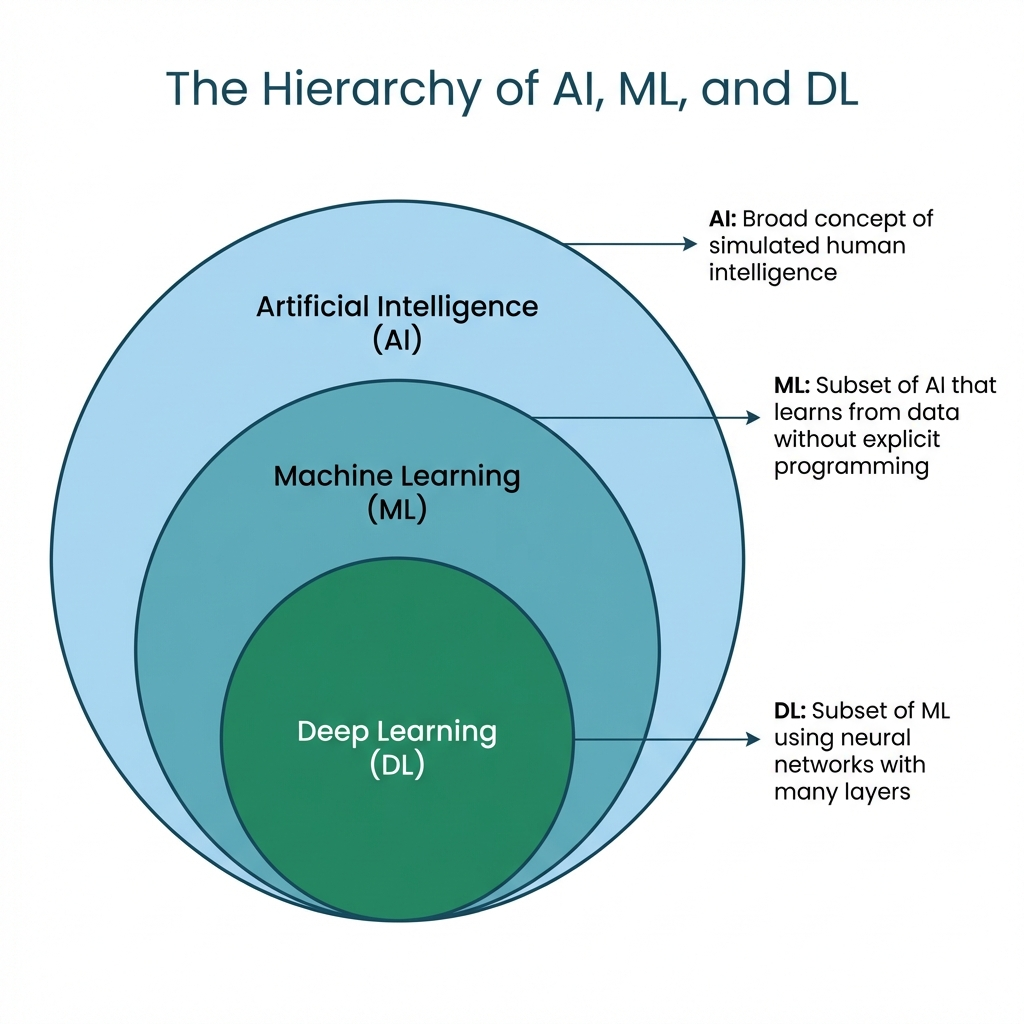
\includegraphics[width=0.6\textwidth]{ai_ml_relationship.png}
	\caption{แผนภาพแสดงความสัมพันธ์เชิงโครงสร้างระหว่าง AI, Machine Learning และ Deep Learning}
	\label{fig:ai_ml_rel}
\end{figure}

เพื่อให้เข้าใจบทบาทของ Machine Learning ในการขับเคลื่อน AI ในโลกความเป็นจริง ได้ดียิ่งขึ้น สามารถพิจารณากรณีศึกษาใน 5 อุตสาหกรรมหลัก ดังภาพประกอบ \ref{fig:ml_apps} และรายละเอียดดังนี้

\begin{figure}[!h]
	\centering
	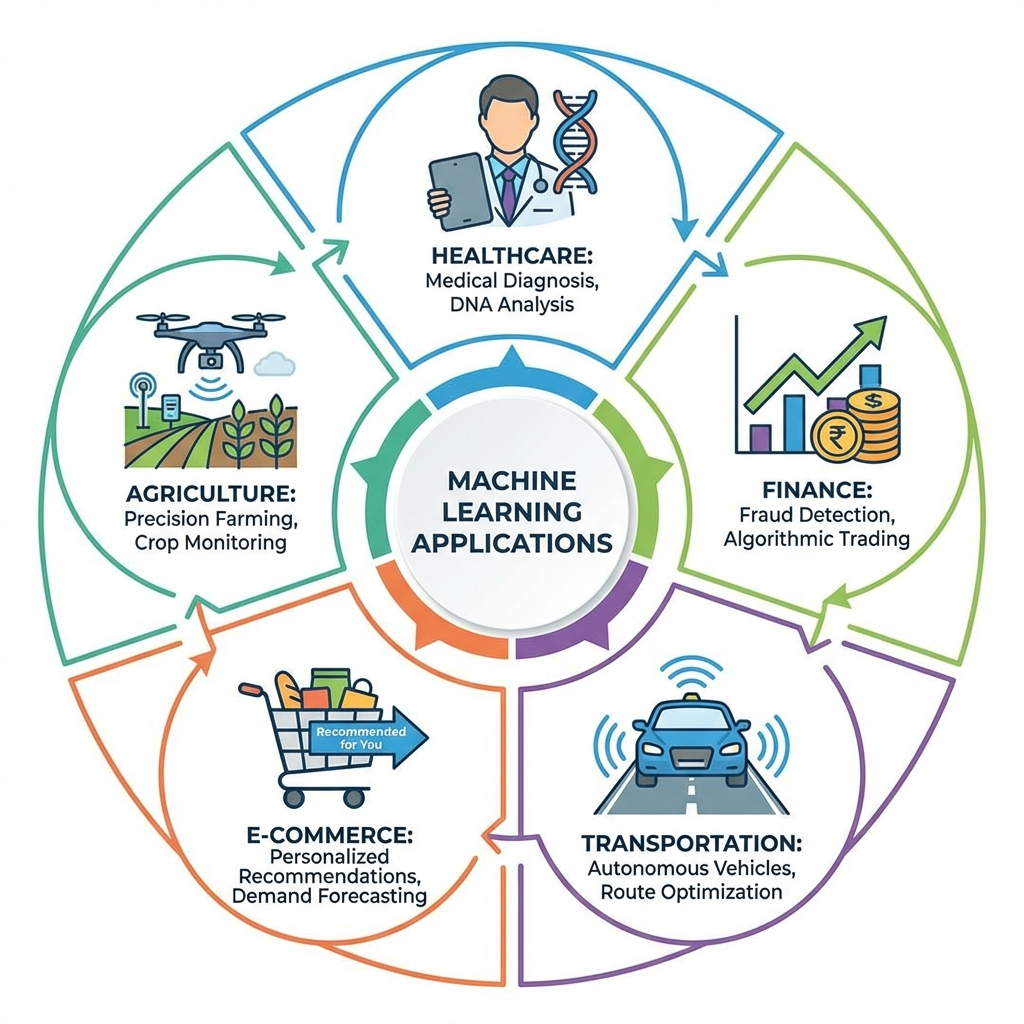
\includegraphics[width=0.6\textwidth]{ml_applications_collage.png}
	\caption{ตัวอย่างการประยุกต์ใช้ Machine Learning ใน 5 อุตสาหกรรมหลัก}
	\label{fig:ml_apps}
\end{figure}

\subsection{กรณีศึกษาการประยุกต์ใช้ (Case Studies)}

\begin{enumerate}
	\item \textbf{ด้านการแพทย์: การวินิจฉัยโรคด้วยภาพถ่าย (Cancer Detection)}
	
	ในอดีต แพทย์ต้องใช้ประสบการณ์ในการอ่านฟิล์มเอ็กซเรย์เพื่อหาจุดผิดปกติ ปัจจุบันมีการใช้ Deep Learning (CNN) เรียนรู้จากภาพถ่ายทางการแพทย์นับล้านภาพ เพื่อช่วยตรวจจับมะเร็งผิวหนังหรือความผิดปกติในปอดได้ด้วยความแม่นยำสูง ซึ่งช่วยลดความผิดพลาดและเพิ่มโอกาสในการรักษาผู้ป่วยได้ทันท่วงที
	
	\item \textbf{ด้านการเงิน: การตรวจจับการฉ้อโกง (Fraud Detection)}
	
	สถาบันการเงินใช้ ML ในการวิเคราะห์รูปแบบการทำธุรกรรมแบบเรียลไทม์ หากระบบตรวจพบพฤติกรรมที่ผิดปกติ เช่น การรูดบัตรเครดิตในสถานที่ที่ไม่คุ้นเคยหรือยอดเงินที่สูงผิดปกติ ระบบจะระงับการทำธุรกรรมชั่วคราวและแจ้งเตือนเจ้าของบัญชีทันที ซึ่งเป็นการป้องกันความเสียหายทางการเงินได้อย่างมีประสิทธิภาพ
	
	\item \textbf{ด้านการคมนาคม: รถยนต์ขับเคลื่อนอัตโนมัติ (Autonomous Vehicles)}
	
	ระบบขับเคลื่อนอัตโนมัติของรถยนต์ เช่น Tesla หรือ Waymo ทำงานโดยการประมวลผลข้อมูลจากกล้องและเซนเซอร์รอบคันผ่านอัลกอริทึม ML เพื่อตัดสินใจในการบังคับเลี้ยว เบรก หรือเร่งความเร็ว โดยเรียนรู้จากสถานการณ์ขับขี่จริงหลายล้านกิโลเมตร ทำให้รถยนต์สามารถเดินทางได้อย่างปลอดภัยโดยไม่ต้องพึ่งพามนุษย์
	
	\item \textbf{ด้านพาณิชย์อิเล็กทรอนิกส์: ระบบแนะนำสินค้า (Recommender Systems)}
	
	แพลตฟอร์มอย่าง Netflix หรือ Amazon ใช้เทคนิค Collaborative Filtering ในการวิเคราะห์ประวัติการซื้อและการเข้าชมของลูกค้า เพื่อนำเสนอสินค้าหรือภาพยนตร์ที่ "ตรงใจ" ผู้ใช้แต่ละคนมากที่สุด ซึ่งไม่เพียงแต่เพิ่มความพึงพอใจให้กับลูกค้า แต่ยังช่วยเพิ่มยอดขายให้กับธุรกิจได้อย่างมหาศาล
	
	\item \textbf{ด้านการเกษตร: เกษตรอัจฉริยะ (Precision Agriculture)}
	
	เกษตรกรสมัยใหม่ใช้โดรนและเซนเซอร์ IoT เก็บข้อมูลความชื้นในดินและสภาพอากาศ ส่งให้ ML วิเคราะห์เพื่อพยากรณ์โรคพืชและแมลงศัตรูพืช รวมไปถึงการคำนวณปริมาณน้ำและปุ๋ยที่เหมาะสมสำหรับพืชแต่ละต้น ช่วยลดต้นทุนการผลิตและเพิ่มผลผลิตต่อไร่ให้สูงขึ้นอย่างยั่งยืน
\end{enumerate}
\section{ประเภทของการเรียนรู้ของเครื่อง}

การเรียนรู้ของเครื่อง (Machine Learning) สามารถจำแนกออกเป็น 3 ประเภทหลักตามลักษณะของข้อมูลที่ใช้ในการเรียนรู้และกลไกการให้ผลป้อนกลับ (Feedback Mechanism) ดังนี้

\begin{enumerate}
    \item \textbf{การเรียนรู้แบบมีผู้สอน (Supervised Learning)}
    
    เป็นการสอนให้คอมพิวเตอร์เรียนรู้จากข้อมูลที่มีการระบุคำตอบ (Labeled Data) เอาไว้ล่วงหน้า เปรียบเสมือนการที่มี "ครู" คอยเฉลยข้อสอบให้เรียนรู้ เป้าหมายคือการสร้างโมเดลที่สามารถทำนายคำตอบของข้อมูลชุดใหม่ที่ไม่เคยเห็นมาก่อนได้ ตัวอย่างเช่น \textbf{การกรองอีเมลขยะ (Spam Filtering)} ที่มึการระบุว่าอีเมลฉบับไหนเป็น "ขยะ" หรือ "ไม่เป็นขยะ" เพื่อให้ระบบเรียนรู้ที่จะแยกแยะอีเมลใหม่ๆ ได้เอง หรือ \textbf{การทำนายราคาบ้าน} จากประวัติการซื้อขายที่ผ่านมา

    \item \textbf{การเรียนรู้แบบไม่มีผู้สอน (Unsupervised Learning)}
    
    เป็นการเรียนรู้จากข้อมูลดิบที่ไม่มีคำตอบระบุไว้ (Unlabeled Data) คอมพิวเตอร์ต้องทำหน้าที่ค้นหาโครงสร้าง รูปแบบ หรือความสัมพันธ์ที่ซ่อนอยู่ด้วยตัวเอง เปรียบเสมือนการให้เด็กเรียนรู้ที่จะแยกประเภทของเล่นด้วยตัวเองโดยไม่มีใครบอก ตัวอย่างที่พบบ่อยคือ \textbf{การแบ่งกลุ่มลูกค้า (Customer Segmentation)} ในทางการตลาด โดยระบบจะจัดกลุ่มลูกค้าที่มีพฤติกรรมคล้ายคลึงกันให้อยู่กลุ่มเดียวกัน เพื่อให้ธุรกิจสามารถนำเสนอโปรโมชันที่เหมาะสมกับแต่ละกลุ่มได้

    \item \textbf{การเรียนรู้แบบเสริมกำลัง (Reinforcement Learning)}
    
    เป็นการเรียนรู้จากการปฏิสัมพันธ์กับสภาพแวดล้อมผ่านกระบวนการ "ลองผิดลองถูก" (Trial and Error) โดยมี "รางวัล" (Reward) หรือ "บทลงโทษ" (Punishment) เป็นตัวกำหนดพฤติกรรม เป้าหมายคือการหาวิธีการตัดสินใจ (Policy) ที่ทำให้ได้รับรางวัลสะสมสูงสุด ตัวอย่างที่ชัดเจนคือ \textbf{การฝึกหุ่นยนต์ให้เดิน} หรือ \textbf{AI เล่นเกม} ที่ระบบจะเรียนรู้ว่าการเคลื่อนไหวแบบใดทำให้ชนะหรือแพ้
\end{enumerate}

เพื่อให้เห็นภาพรวมความแตกต่างและความสัมพันธ์ของทั้ง 3 ประเภท สามารถพิจารณาได้จากภาพประกอบ \ref{fig:ml_types}

\begin{figure}[h]
    \centering
    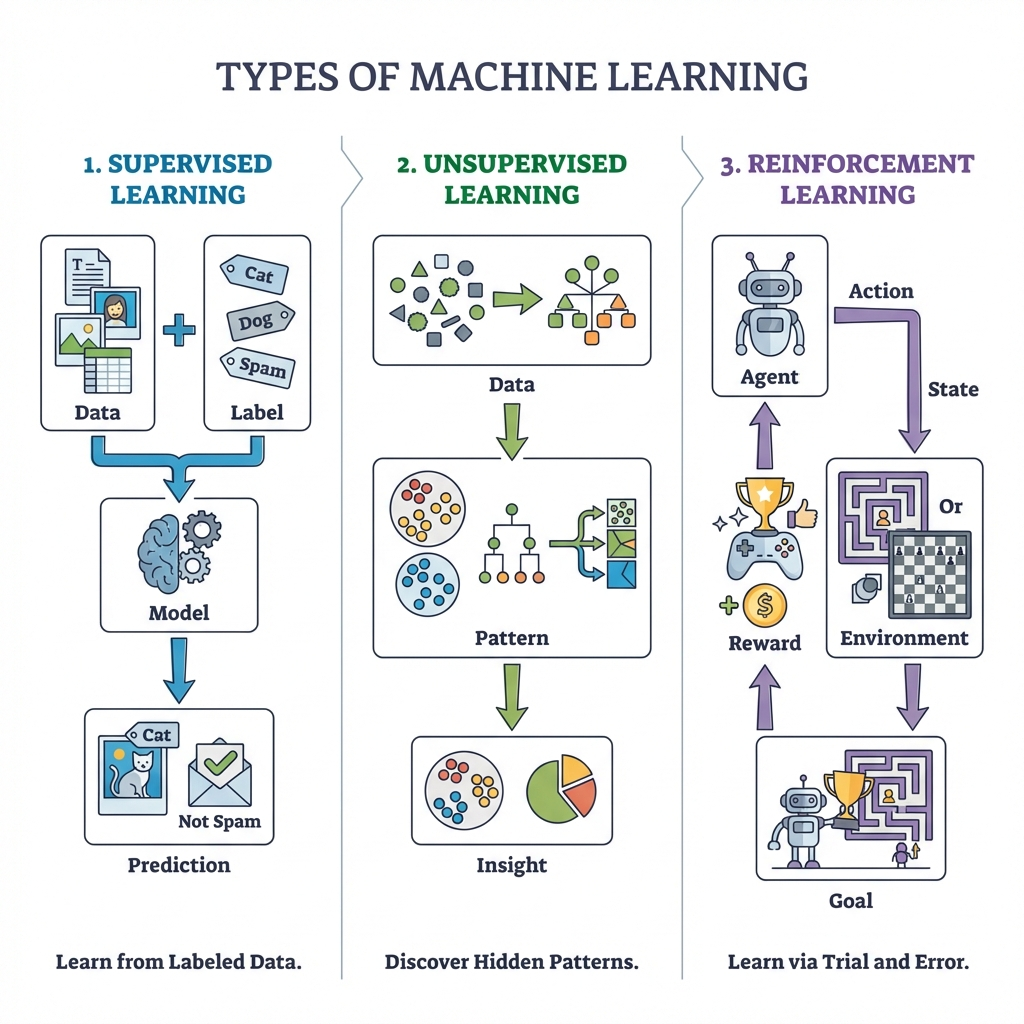
\includegraphics[width=0.8\textwidth]{ml_types_diagram.png}
    \caption{โครงสร้างประเภทของการเรียนรู้ของเครื่อง: Supervised, Unsupervised, และ Reinforcement Learning}
    \label{fig:ml_types}
\end{figure}



\section{กระบวนการวิเคราะห์ข้อมูลและการสร้างโมเดล}

กระบวนการวิเคราะห์ข้อมูลและการสร้างโมเดล (Data Analysis and Model Building Process) เป็นหัวใจสำคัญของวิทยาการข้อมูล (Data Science) และการเรียนรู้เชิงสถิติ (Statistical Learning) กระบวนการดังกล่าวมิได้เป็นเพียงการคำนวณทางคณิตศาสตร์เพียงอย่างเดียว แต่เป็นวัฒจักรที่มีโครงสร้างชัดเจน ประกอบด้วยขั้นตอนที่สัมพันธ์กันอย่างเป็นระบบ ตั้งแต่การกำหนดปัญหา การรวบรวมและจัดเตรียมข้อมูล การวิเคราะห์เชิงสำรวจ การสร้างโมเดล ไปจนถึงการประเมินและนำโมเดลไปใช้งานจริง

กรอบการทำงานที่ได้รับการยอมรับในระดับสากลสำหรับกระบวนการนี้คือ \textbf{CRISP-DM} (Cross-Industry Standard Process for Data Mining) ซึ่งนำเสนอวัฏจักรการทำงาน 6 ระยะที่เวียนซ้ำและส่งผลย้อนกลับซึ่งกันและกัน ดังแสดงในภาพประกอบ \ref{fig:crisp_dm}

\begin{figure}[h]
    \centering
    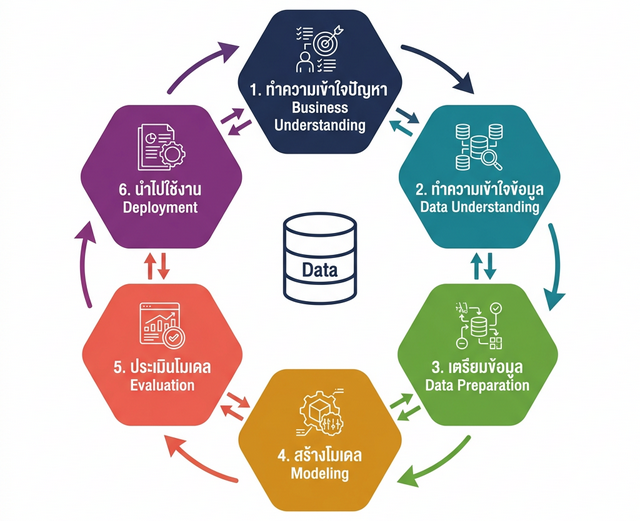
\includegraphics[width=0.75\textwidth]{CH1_crisp_dm.png}
    \caption{วัฏจักรกระบวนการ CRISP-DM สำหรับการวิเคราะห์ ข้อมูลและการสร้างโมเดล}
    \label{fig:crisp_dm}
\end{figure}

%--------------------------------------------------
\subsection{ระยะที่ 1: การทำความเข้าใจปัญหาทางธุรกิจหรือการวิจัย}

ขั้นตอนแรกและสำคัญที่สุดของกระบวนการคือการทำความเข้าใจ \textbf{วัตถุประสงค์} ของปัญหาอย่างชัดเจน ก่อนที่จะดำเนินการใด ๆ ทางสถิติหรือเทคนิค นักวิทยาศาสตร์ข้อมูลจำเป็นต้องตอบคำถามสำคัญ 3 ข้อ ได้แก่

\begin{enumerate}
    \item \textbf{ปัญหาคืออะไร?} --- ต้องการทำนาย จำแนก จัดกลุ่ม หรือค้นหาความสัมพันธ์?
    \item \textbf{ผลลัพธ์ที่ต้องการคืออะไร?} --- ตัวชี้วัดความสำเร็จของโมเดลคืออะไร?
    \item \textbf{ข้อจำกัดมีอะไรบ้าง?} --- ทรัพยากร เวลา และข้อจำกัดทางจริยธรรม
\end{enumerate}

การกำหนดปัญหาที่ชัดเจนจะนำไปสู่การเลือกประเภทของโมเดลที่เหมาะสม เช่น หากตัวแปรตามเป็นค่าต่อเนื่อง ควรใช้ \textbf{การวิเคราะห์การถดถอย (Regression Analysis)} หากเป็นการจำแนกประเภทควรใช้ \textbf{Classifier} และหากไม่มีตัวแปรตามกำหนดไว้ควรใช้ \textbf{การเรียนรู้แบบไม่มีผู้สอน (Unsupervised Learning)}

%--------------------------------------------------
\subsection{ระยะที่ 2: การรวบรวมและทำความเข้าใจข้อมูล}

หลังจากกำหนดปัญหาได้แล้ว ขั้นตอนต่อไปคือการรวบรวมข้อมูล (Data Collection) และการวิเคราะห์เชิงสำรวจ (Exploratory Data Analysis: EDA) กระบวนการนี้ครอบคลุม

\begin{itemize}
    \item \textbf{การวิเคราะห์สถิติเชิงพรรณนา (Descriptive Statistics)} --- ได้แก่ ค่าเฉลี่ย ค่ามัธยฐาน ส่วนเบี่ยงเบนมาตรฐาน และเปอร์เซนไทล์ เพื่อสรุปลักษณะทั่วไปของข้อมูล
    \item \textbf{การตรวจสอบการแจกแจงของข้อมูล (Distribution Analysis)} --- โดยใช้ Histogram, Box Plot, หรือ Q-Q Plot เพื่อตรวจสอบว่าข้อมูลเป็นแบบปกติหรือเบ้
    \item \textbf{การวิเคราะห์ความสัมพันธ์ระหว่างตัวแปร (Correlation Analysis)} --- ใช้ Scatter Plot Matrix หรือ Heatmap เพื่อค้นหาความสัมพันธ์ระหว่างตัวแปรอิสระและตัวแปรตาม
    \item \textbf{การตรวจจับค่าผิดปกติและข้อมูลสูญหาย (Outlier \& Missing Data Detection)} --- ซึ่งเป็นปัญหาที่พบได้บ่อยในข้อมูลจริงและส่งผลกระทบอย่างมากต่อประสิทธิภาพของโมเดล
\end{itemize}

%--------------------------------------------------
\subsection{ระยะที่ 3: การเตรียมข้อมูล}

การเตรียมข้อมูล (Data Preparation หรือ Data Preprocessing) มักใช้เวลาถึง 60--80\% ของกระบวนการทั้งหมด เนื่องจากข้อมูลในโลกความเป็นจริงมักมีปัญหาเหล่านี้ร่วมด้วย

\begin{myBox}[]{ขั้นตอนหลักในการเตรียมข้อมูล}{}
\begin{enumerate}
    \item \textbf{การจัดการข้อมูลสูญหาย (Missing Value Handling)} \\
    วิธีที่นิยมได้แก่ การลบแถวที่มีข้อมูลสูญหาย (Listwise Deletion) การแทนค่าด้วยค่าเฉลี่ยหรือค่ามัธยฐาน (Mean/Median Imputation) หรือการใช้โมเดลทำนายค่าสูญหาย (Model-based Imputation)

    \item \textbf{การแปลงขนาดข้อมูล (Feature Scaling)} \\
    อัลกอริทึมหลายตัว เช่น K-Nearest Neighbors (KNN) หรือ Support Vector Machine (SVM) มีความไวต่อขนาดของตัวแปร จึงจำเป็นต้องทำ \textbf{Standardization} หรือ \textbf{Min-Max Normalization} โดยมีสูตรดังนี้
    \[
        z_i = \frac{x_i - \bar{x}}{s}, \qquad
        x_i^{*} = \frac{x_i - x_{\min}}{x_{\max} - x_{\min}}
    \]

    \item \textbf{การเข้ารหัสตัวแปรจัดประเภท (Categorical Encoding)} \\
    แปลงตัวแปรเชิงคุณภาพให้อยู่ในรูปแบบตัวเลขโดยใช้ \textit{One-Hot Encoding} หรือ \textit{Label Encoding} เพื่อให้อัลกอริทึมสามารถประมวลผลได้

    \item \textbf{การคัดเลือกและสร้างตัวแปร (Feature Selection \& Engineering)} \\
    การเลือกเฉพาะตัวแปรที่มีอิทธิพลต่อตัวแปรตามอย่างมีนัยสำคัญ โดยใช้เทคนิค เช่น Correlation Threshold, Variance Inflation Factor (VIF), หรือ Recursive Feature Elimination (RFE)
\end{enumerate}
\end{myBox}

%--------------------------------------------------
\subsection{ระยะที่ 4: การสร้างและฝึกโมเดล}

ในระยะนี้ ข้อมูลที่ผ่านการเตรียมแล้วจะถูกแบ่งออกเป็น 2 ส่วนตามหลักการมาตรฐาน ได้แก่ \textbf{ชุดข้อมูลฝึกสอน (Training Set)} และ \textbf{ชุดข้อมูลทดสอบ (Test Set)} โดยทั่วไปจะแบ่งในสัดส่วน 70:30 หรือ 80:20

\[
    \mathcal{D} = \mathcal{D}_{\text{train}} \cup \mathcal{D}_{\text{test}}, \quad
    \mathcal{D}_{\text{train}} \cap \mathcal{D}_{\text{test}} = \emptyset
\]

\noindent
จากนั้นเลือกอัลกอริทึมที่เหมาะสมกับลักษณะของปัญหาและข้อมูล โดยพิจารณาจากเกณฑ์ดังตาราง \ref{T:model_selection_guide}

\begin{table}[h]
\centering
\caption{แนวทางการเลือกโมเดลตามลักษณะของปัญหาและข้อมูล}
\label{T:model_selection_guide}
\begin{tabular}{|l|l|l|}
\hline
\textbf{ประเภทปัญหา} & \textbf{ลักษณะข้อมูล} & \textbf{โมเดลที่แนะนำ} \\ \hline
การพยากรณ์ค่าต่อเนื่อง & ความสัมพันธ์เชิงเส้น & Linear Regression \\ \hline
การพยากรณ์ค่าต่อเนื่อง & ความสัมพันธ์ไม่เชิงเส้น & Random Forest, XGBoost \\ \hline
การจำแนกประเภท (2 กลุ่ม) & ข้อมูลตัวเลข & Logistic Regression, SVM \\ \hline
การจำแนกประเภท (หลายกลุ่ม) & ข้อมูลผสม & Decision Tree, Random Forest \\ \hline
การจัดกลุ่ม & ไม่มี Label & K-Means, DBSCAN \\ \hline
การวิเคราะห์อนุกรมเวลา & ข้อมูลเวลาต่อเนื่อง & ARIMA, LSTM \\ \hline
\end{tabular}
\end{table}

กระบวนการฝึกโมเดล (Model Training) คือการหาค่าพารามิเตอร์ $\boldsymbol{\theta}^*$ ที่ \textbf{ลดค่าฟังก์ชันสูญเสีย (Loss Function)} $\mathcal{L}(\boldsymbol{\theta})$ ให้น้อยที่สุด ดังสมการ

\[
    \boldsymbol{\theta}^* = \underset{\boldsymbol{\theta}}{\arg\min} \; \mathcal{L}(\boldsymbol{\theta}) = \underset{\boldsymbol{\theta}}{\arg\min} \; \frac{1}{n}\sum_{i=1}^{n} \ell\!\left(y_i,\, f(\mathbf{x}_i; \boldsymbol{\theta})\right)
\]

\noindent
โดย $\ell(\cdot)$ คือฟังก์ชันสูญเสียรายตัวอย่าง เช่น Mean Squared Error (MSE) สำหรับการถดถอย หรือ Cross-Entropy Loss สำหรับการจำแนกประเภท

%--------------------------------------------------
\subsection{ระยะที่ 5: การประเมินประสิทธิภาพโมเดล}

การประเมินโมเดลที่ถูกต้องต้องอาศัยตัวชี้วัดที่เหมาะสมกับประเภทของงาน และต้องดำเนินการบนชุดข้อมูลที่โมเดลไม่เคยเห็นมาก่อน (Holdout Set) เพื่อประเมิน \textbf{ความสามารถในการ Generalize} ของโมเดล

\begin{itemize}
    \item \textbf{สำหรับงาน Regression}: ใช้ Root Mean Squared Error (RMSE), Mean Absolute Error (MAE) และสัมประสิทธิ์การตัดสินใจ $R^2$
    \[
        \text{RMSE} = \sqrt{\frac{1}{n}\sum_{i=1}^{n}(y_i - \hat{y}_i)^2}, \qquad
        R^2 = 1 - \frac{\sum_{i=1}^{n}(y_i - \hat{y}_i)^2}{\sum_{i=1}^{n}(y_i - \bar{y})^2}
    \]

    \item \textbf{สำหรับงาน Classification}: ใช้ Accuracy, Precision, Recall และ F1-Score ซึ่งคำนวณจาก Confusion Matrix

    \item \textbf{การตรวจสอบ Bias--Variance Tradeoff}: เพื่อตรวจสอบว่าโมเดลอยู่ในสภาวะ \textit{Overfitting} (ค่าความผิดพลาดในชุดฝึกต่ำ แต่สูงในชุดทดสอบ) หรือ \textit{Underfitting} (ค่าความผิดพลาดสูงทั้งสองชุด)

    \item \textbf{การทำ Cross-Validation}: ใช้ $k$-Fold Cross-Validation เพื่อประเมินประสิทธิภาพโมเดลอย่างรอบด้านโดยลดผลกระทบจากการสุ่มแบ่งข้อมูล
\end{itemize}

%--------------------------------------------------
\subsection{ระยะที่ 6: การนำโมเดลไปใช้งาน}

ระยะสุดท้ายคือการนำโมเดลที่ผ่านการประเมินแล้วไปติดตั้งในระบบจริง (Model Deployment) การดำเนินการในระยะนี้ประกอบด้วย

\begin{enumerate}
    \item \textbf{การบรรจุโมเดลเป็น API} (Model Serving) เพื่อให้ระบบอื่น ๆ สามารถเรียกใช้งานได้ผ่าน Web Service
    \item \textbf{การติดตามและการดูแลรักษาโมเดล} (Model Monitoring \& Maintenance) โดยตรวจสอบว่าประสิทธิภาพของโมเดลยังคงอยู่ในระดับที่ยอมรับได้เมื่อเวลาผ่านไป
    \item \textbf{การอัปเดตโมเดล} (Model Retraining) เมื่อพฤติกรรมของข้อมูลเปลี่ยนแปลงไปจากเดิม ซึ่งเรียกปรากฏการณ์นี้ว่า \textit{Data Drift} หรือ \textit{Concept Drift}
\end{enumerate}

\begin{myLimit}[]{ข้อควรระวังในกระบวนการวิเคราะห์ข้อมูลและสร้างโมเดล}{}
\begin{itemize}
    \item \textbf{Data Leakage} --- การที่ข้อมูลจากชุดทดสอบ ``รั่วไหล'' เข้าไปในกระบวนการฝึกสอน ทำให้ผลการประเมินโมเดลสูงเกินจริง
    \item \textbf{Class Imbalance} --- เมื่อกลุ่มข้อมูลมีความไม่สมดุล เช่น ผู้ป่วยโรคหายาก 1\% ต่อผู้ไม่ป่วย 99\% โมเดลอาจให้ Accuracy สูง แต่ Recall ต่ำมาก ต้องใช้เทคนิคเฉพาะเช่น SMOTE หรือ Class Weighting
    \item \textbf{Multicollinearity} --- ตัวแปรอิสระที่มีความสัมพันธ์กันสูงจะทำให้การประมาณค่าสัมประสิทธิ์ไม่เสถียร ต้องตรวจสอบด้วย Variance Inflation Factor (VIF $> 10$ ถือว่ามีปัญหา)
    \item \textbf{ความเป็นตัวแทนของข้อมูล} --- ข้อมูลที่ใช้ฝึกสอนต้องเป็นตัวแทนของประชากรที่โมเดลจะถูกนำไปใช้จริง มิฉะนั้นโมเดลจะมีความลำเอียง (Bias) อย่างเป็นระบบ
\end{itemize}
\end{myLimit}

\begin{exmp}
    โรงพยาบาลศูนย์ต้องการพัฒนาระบบทำนายความยาวนานในการนอนโรงพยาบาล (Length of Stay: LOS) ของผู้ป่วยโรคปอดบวม เพื่อวางแผนการจัดสรรเตียงและทรัพยากรทางการแพทย์ล่วงหน้า สรุปกระบวนการทั้ง 6 ระยะตามกรอบ CRISP-DM ดังนี้

    \begin{enumerate}
        \item \textbf{ทำความเข้าใจปัญหา}: ตัวแปรตามคือ LOS (จำนวนวัน, ต่อเนื่อง) $\Rightarrow$ ปัญหาการถดถอย
        \item \textbf{ทำความเข้าใจข้อมูล}: รวบรวมข้อมูลผู้ป่วย 500 ราย ตัวแปร ได้แก่ อายุ เพศ BMI ระดับออกซิเจนในเลือด (SpO$_2$) จำนวนโรคประจำตัว และผลการตรวจ CBC
        \item \textbf{เตรียมข้อมูล}: จัดการค่าสูญหาย 3.2\% ด้วย Median Imputation, ทำ Standardization ตัวแปรต่อเนื่อง, เข้ารหัสตัวแปร เพศ ด้วย Label Encoding
        \item \textbf{สร้างโมเดล}: เปรียบเทียบ Linear Regression, Random Forest และ XGBoost โดยแบ่งข้อมูล 80:20 และใช้ 5-Fold Cross-Validation
        \item \textbf{ประเมินโมเดล}: Random Forest ให้ผลดีที่สุดด้วย RMSE $= 1.8$ วัน และ $R^2 = 0.87$
        \item \textbf{นำไปใช้งาน}: พัฒนา Dashboard ให้พยาบาลกรอกข้อมูลผู้ป่วยและระบบแสดงการพยากรณ์ LOS แบบ real-time
    \end{enumerate}
\end{exmp}

\textbf{สรุป:} กระบวนการวิเคราะห์ข้อมูลและการสร้างโมเดลเป็นวัฏจักรที่ต้องการความรู้แบบสหวิทยาการ ทั้งสถิติศาสตร์ วิทยาการคอมพิวเตอร์ และความเข้าใจในบริบทของปัญหา การดำเนินการแต่ละระยะอย่างรอบคอบและเป็นระบบเป็นกุญแจสำคัญที่ทำให้โมเดลที่ได้มีความน่าเชื่อถือและสามารถนำไปประยุกต์ใช้ได้อย่างมีประสิทธิผลในโลกความเป็นจริง

\section{เครื่องมือสำหรับการเรียนรู้เชิงสถิติ}






%\chapter{การเรียนรู้แบบมีผู้สอน}
%\chapter{การเรียนรู้แบบไม่มีผู้สอน}
%\chapter{เทคนิคการวิเคราะห์การถดถอย}
%\chapter{เทคนิคการเรียนรู้เชิงสถิติ}
%\chapter{การประเมินผลและการปรับปรุงประสิทธิภาพของแบบจำลอง}










\newpage
%\RefChapter